\documentclass[11pt]{article}
\usepackage[super,square,comma]{natbib}
\usepackage[letterpaper, margin=1.25in]{geometry}
\usepackage{tikz}
\usepackage{lipsum}
\usepackage{setspace}
\usepackage{enumerate}
\usepackage[inline, shortlabels]{enumitem}
\usepackage{amsmath}
\numberwithin{equation}{section}

\usepackage{csquotes}
\usepackage{graphicx}
\usepackage{authblk}
\usepackage[labelfont=bf]{caption}
\usepackage{subcaption}

\usepackage{fancyhdr}
\pagestyle{fancy}
\lhead{Team 93463}
\chead{Multi-hop, HF Radio Propagation Near S. America}
\rhead{Page \thepage\ of \pageref{LastPage}}
\setlength{\headheight}{14pt}

\usepackage{lastpage}

\renewcommand{\thefootnote}{\arabic{footnote}}
\newcommand{\cn}{$^{\text{[citation needed]}}$} %citation needed

% %%% Title Page Author Stuff %%%
% \renewcommand*{\Authsep}{, }
% \renewcommand*{\Authand}{, }
% \renewcommand*{\Authands}{, }
% \renewcommand*{\Affilfont}{\normalsize\normalfont}
% % \renewcommand*{\Authfont}{\bfseries}    % make author names boldface    
% \setlength{\affilsep}{1em}   % set the space between author and affiliation

% \newsavebox\affbox

% \author[1]{Colin M. Adams}
% \author[1]{Rachel L. Barcklay}
% \author[1,2]{Carla J. Becker}
% \affil[1]{%
%   \savebox\affbox{\Affilfont Department of Physics, Harvey Mudd College}%
%   \parbox[t]{\wd\affbox}{\protect\centering Department of Physics, Harvey Mudd College}} 
% \affil[2]{Department of Chemistry, Harvey Mudd College \par Claremont, CA 91711}



%%%%%%%%%%%%%%%%%%%%%%%
\renewcommand{\baselinestretch}{2}
\newcommand{\shrug}[1][]{%
\begin{tikzpicture}[baseline,x=0.8\ht\strutbox,y=0.8\ht\strutbox,line width=0.125ex,#1]
\def\arm{(-2.5,0.95) to (-2,0.95) (-1.9,1) to (-1.5,0) (-1.35,0) to (-0.8,0)};
\draw \arm;
\draw[xscale=-1] \arm;
\def\headpart{(0.6,0) arc[start angle=-40, end angle=40,x radius=0.6,y radius=0.8]};
\draw \headpart;
\draw[xscale=-1] \headpart;
\def\eye{(-0.075,0.15) .. controls (0.02,0) .. (0.075,-0.15)};
\draw[shift={(-0.3,0.8)}] \eye;
\draw[shift={(0,0.85)}] \eye;
% draw mouth
\draw (-0.1,0.2) to [out=15,in=-100] (0.4,0.95); 
\end{tikzpicture}}


\title{
    \textsc{{Multi-hop, High-Frequency Radio Propagation Near South America}}
    }

\author{\Large Team 93463}
\date{\today}
        

\begin{document}
%%%%%%%%%%%%%%%%%%%%%%%%%%%%%%%%%%%%%%%%%%%%%%%%%%%%%%%%%%%%%%%%%%%%%%
% Title Page
%%%%%%%%%%%%%%%%%%%%%%%%%%%%%%%%%%%%%%%%%%%%%%%%%%%%%%%%%%%%%%%%%%%%%%
    \singlespacing %sets spacing of abstract to single
    \clearpage 
    \maketitle
    \thispagestyle{empty} %gets rid of page number at bottom 

\begin{abstract}
    \shrug\cite{townsend2000modern}
\end{abstract}
\newpage

%%%%%%%%%%%%%%%%%%%%%%%%%%%%%%%%%%%%%%%%%%%%%%%%%%%%%%%%%%%%%%%%%%%%%
%% Body
%%%%%%%%%%%%%%%%%%%%%%%%%%%%%%%%%%%%%%%%%%%%%%%%%%%%%%%%%%%%%%%%%%%%%
\setcounter{page}{1} %set new page number to 1

\section*{MCM Requirements}

Hi team, here is what we \emph{need} to have in our report (according to the MCM overlords):
\begin{itemize}
    \item Restatement and clarification of the problem
    \item Explain assumptions and rationale/justification
    \item Include your model design and justification
    \item Describe model testing and sensitivity analysis
    \item Discuss the strengths and weaknesses
\end{itemize}

They also claim to judge the quality of our writing. So remember our good friend Williams.

\section{Motivation} % (fold)
\label{sec:motivation}

% section motivation (end)

\section{Introduction} 
\label{sec: intro}

\section{Model} % (fold)
\label{sec:model}

\subsection{Radiowaves} % (fold)
\label{sub:radiowaves}

% subsection radiowaves (end)

\subsection{The Ionosphere} % (fold)
\label{sub:the_ionosphere}

The ionosphere consists of roughly three layers that lie between 75--1000\,km above the Earth's surface:
\begin{enumerate*}[(1)]
    \item the F-region,
    \item the E-region, and
    \item the D-region
\end{enumerate*}; each of these regions has charge-density dependent on the time of year, the sunspots number of sunspots present, the time of day, and the movement of the charged particles\footnote{The study of which has the impressive sounding name of magnetohydrodynamics.}(Figure \ref{fig:struct_ion}). X-rays, ultraviolet light, ejected plasma, and other high energy particles that are released by the sun interact with the atoms in the atmosphere and strip them of electrons.\cite{noauthor_tracking_nodate} The ionosphere interacts heavily with radio waves, mainly through the interaction of these free electrons.\cite{budden1961radio}

Early experiments demonstrated that the electrons in the ionosphere are arranged in approximately horizontal layers, meaning that the number density is a function of height above the Earth's surface. Presumably, these cations are stripped atoms or molecules. Because the ratio between the mass of a proton (the smallest positive charge we could have in the atmosphere) and an electron is on the order of $2\times10^3$, we would expect there must be approximately $5 \times10{-4}$ more cations than electrons.\footnote{This is because the electric field of the propagating radio-waves will have $5 \times10^{-4}$ of the effect on a proton than an electron because $F \propto m$.} If this were the case, the ionosphere would be unstable, due to the large repulsive forces of this unbalanced positive charge. However, due to the ionosphere's empirically determined and stable layers, the ionosphere must be nearly electrically neutral, i.e. there must be an equal number of positive and negative charges per unit volume.\cite{budden1961radio} Consequently, we assume that the radio-waves only interact with the free electrons in the ionosphere.

\begin{figure}[ht]
 \begin{center}
 \begin{subfigure}[b]{0.44\textwidth}
    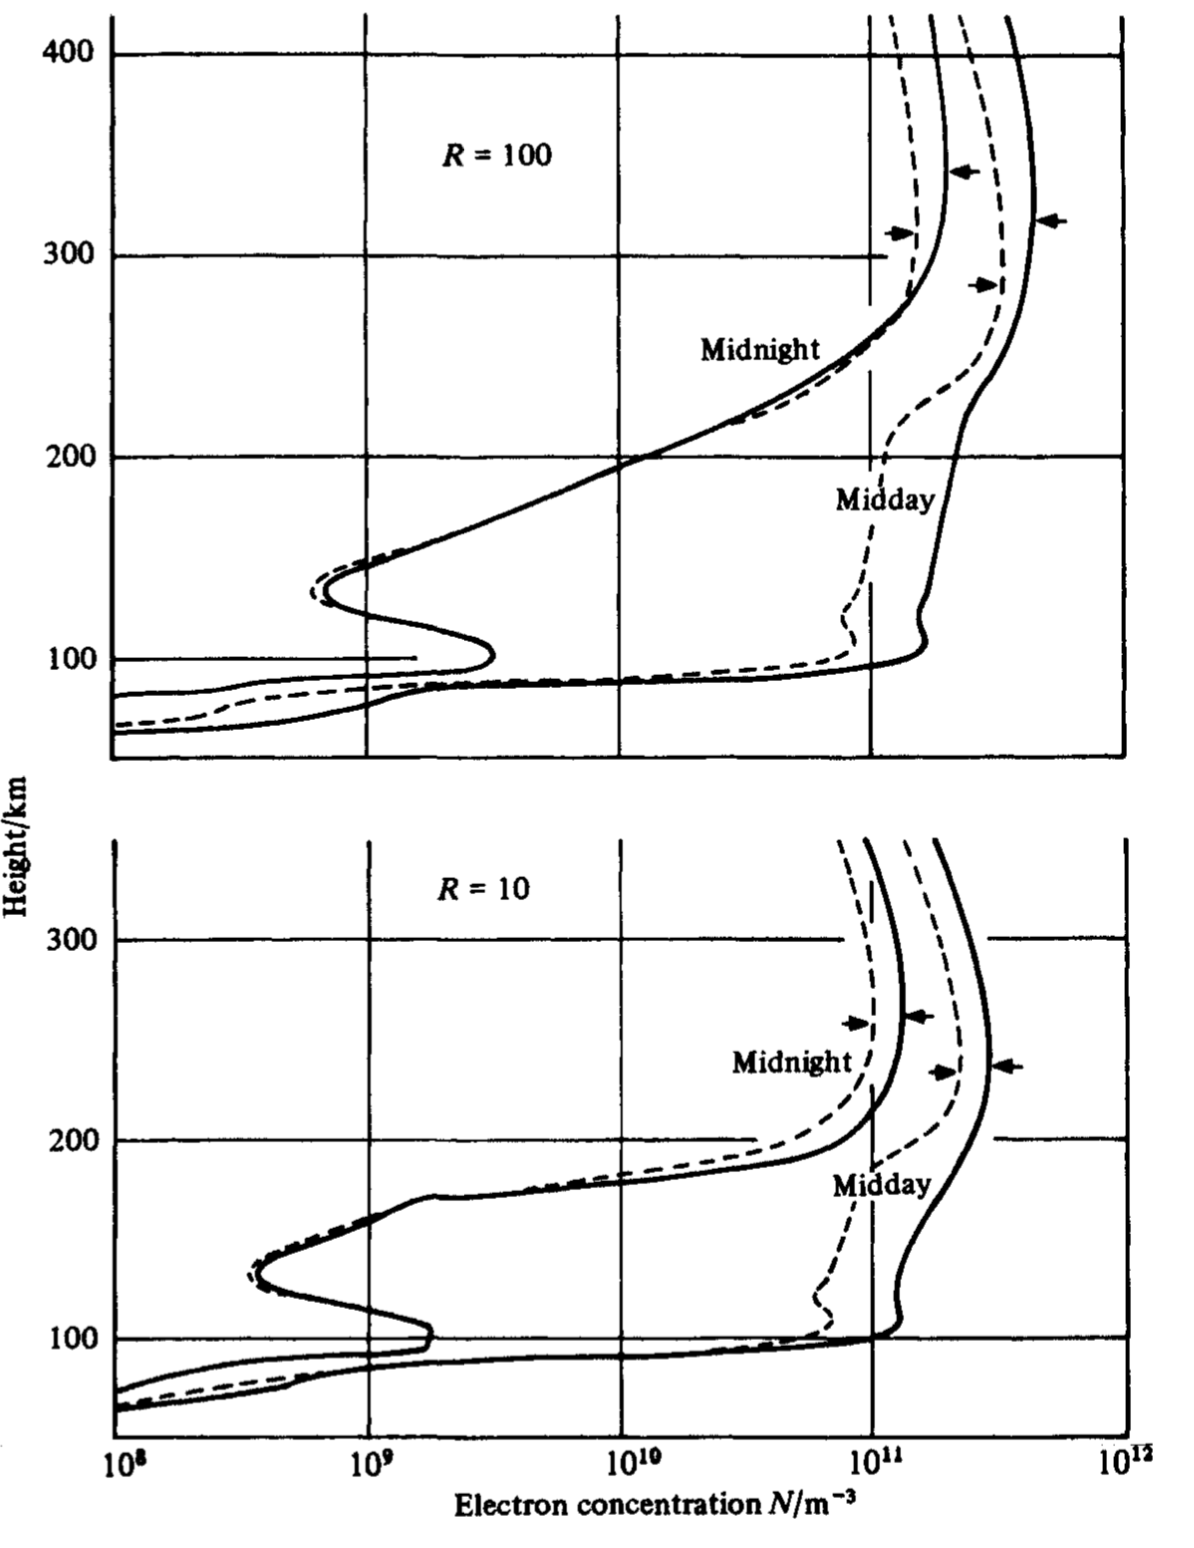
\includegraphics[width = 3in]{figs/structure_iono.png}
         \caption{}
    \label{fig:struct_ion} 
 \end{subfigure}
~
 \begin{subfigure}[b]{0.44\textwidth}
         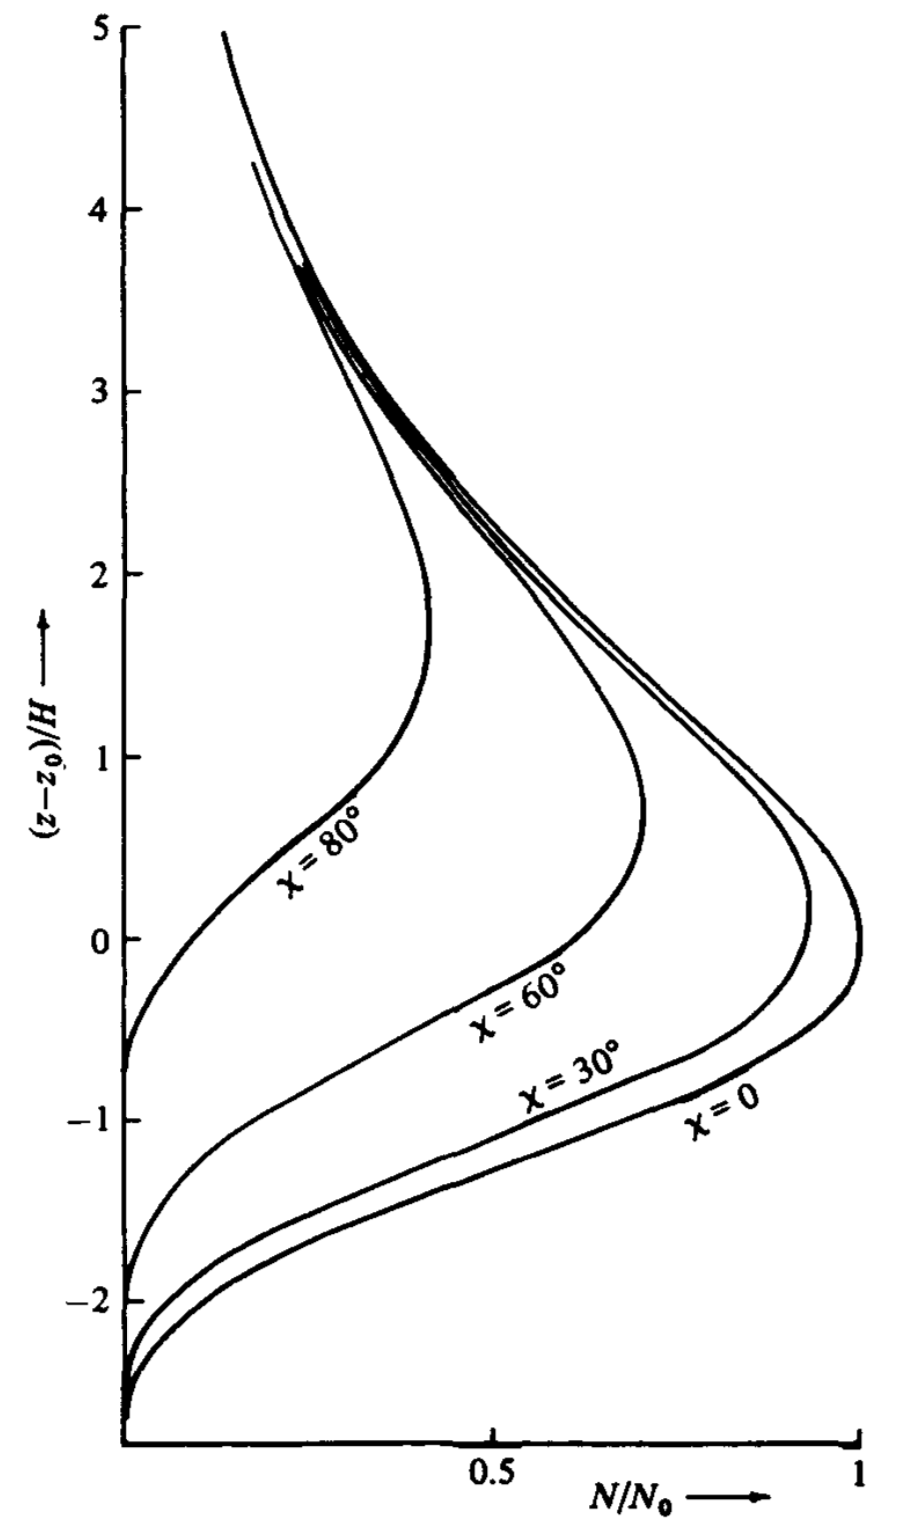
\includegraphics[width = 3.25in]{figs/chapman.png}
          \caption{ }
     \label{fig:chapman}
 \end{subfigure}
 \end{center}
 \caption{\text{(a)} The charge density as a function of height in the ionosphere. It also shows how the ionosphere changes at midnight and noon. Dashed lines are for January while solid lines are for June. Also given is the number of sunspots, $R$, at the time of data collection.  Figure is taken from K.G. Budden (1961).\cite{budden1988propagation} \text{(b)} Contour plot of the Chapman Law for various azimuthal angles. Figure taken from K.G. Budden (1988).\cite{budden1988propagation} }
 \label{fig:elect_density}
\end{figure}

As stated above, at a first approximation, we expect that the electron density, $N$, is only a function of the eight above the earth's surface height, $z$. More compactly, $N = N(z)$. 

    \subsubsection{Electron Density, $N(z)$} % (fold)
    \label{ssub:electron_density}
    Before we can calculate how radio-waves are reflected off of the ionosphere, we must model the ionosphere's electron density. In the early 1930's, a simple model for the electron density as a function was produced called the Chapman Law.\cite{chapman1931b,chapman1931a} 

    If we assume the Earth is constant in composition and temperature (as well as neglect the curvature of the earth\footnote{See \texttt{https://www.tfes.org/} for more information.}), then the density of the atmosphere, $\rho = \rho(z)$, is given by 
    \begin{equation}
        \rho(z) = \rho_0 e^{-M g z/ RT} = \rho_0 e^{- z/\kappa} 
        \label{eq:atm_den}
    \end{equation} where $ \kappa \equiv RT/Mg$, $\rho_0 \equiv \rho(0)$, $M$ is the average molecular weight, $g$ is the gravitational acceleration (assumed constant), $R$ is the universal gas constant,\footnote{Since all of us are ``physicists,'' we feel the need to note the definition of $R$: $R\equiv k_B N_A$ where $k_B$ is Boltzmann's constant and $N_A$ is Avogadro's number.} and $T$ is the temperature. The result of (\ref{eq:atm_den}) comes by balancing the forces acting on infinitesimal layers of atmosphere that, on a whole, is taken to be static and solving the barometric equation.\cite{schroeder1999introduction}
    
    Next, we must find the intensity of the sun that passes through the earth's atmosphere. The intensity of the sun---not surprisingly---decreases as it goes through the atmosphere.\cite{budden1961radio} Since, the sun enters at an angle from the zenith, $\alpha$. By drawing a simple diagram,\footnote{Remember, we have a flat Earth; this is a subtle but important point in this derivation.} we can see that the area normal to the incident radiation of the sun will be a factor of secant too large than the area that the ground actually receives, i.e. $dA = dA_\perp \cos\alpha.$ Since intensity is inversely proportional to $dA$, we will have the relationship of 
    \begin{equation}
        dI = I \sigma \rho \sec(\alpha) \, dz.
        \label{eq:diff_intensity}
    \end{equation}
    where $\sigma$ is a mass coefficient of absorption of the atmosphere. If we plug (\ref{eq:atm_den}) into (\ref{eq:diff_intensity}) and integrate, we get
    \begin{align}
        I(z)&= I_0 \exp\left[ -\sigma \kappa  \rho_0 \sec(\alpha) e^{- z/\kappa}\right] = I_0 \exp\left[ - \sec(\alpha) e^{- (z - z_0)/\kappa}\right]
        \label{eq:inten_v_height}
    \end{align}
    if we (cleverly) define $z_0 \equiv \kappa \ln \left(\sigma \kappa  \rho_0\right)$. The rate of absorption of energy at height $z$ is $\cos(\alpha)(dI/dz)$. If we assume that the rate of production of electrons, $q$, is proportional to this, then we get 
    \begin{equation}
        q(z) = q_0 \exp\left[1 - \frac{z-z_0}{\kappa} - \sec(\alpha) e^{- (z - z_0)/\kappa}\right].
        \label{eq:rate_prod_elec}
    \end{equation}


    \begin{figure}[ht]

    \end{figure}

    Empirically---at least in the D and E-layers of the ionosphere\footnote{In the F-layer, this rate law may be equal to $dN/dt = q - b N$}---the variation of charge density is given by\cite{budden1961radio}
    \begin{equation}
        \frac{dN}{dt} = q - a N^2
        \label{eq:charge_den_rate}
    \end{equation}
    where $a$ is a ``recombination constant.'' In the steady-state solution, where $dN/dt \approx 0$, we have $N = \sqrt{q/a}$ or
    \begin{equation}
        N(z) = N_0 \exp\left[\frac12\left(1 - \frac{z-z_0}{\kappa} - \sec(\alpha) e^{- (z - z_0)/\kappa}\right)\right]
    \end{equation}
    where $N_0$ is a constant we can gather from experimental data. This is the Chapman Law.


    % subsubsection electron_density (end)
    
% subsection the_ionosphere (end)

\subsection{The Ocean} % (fold)
\label{sub:the_ocean}

% subsection the_ocean (end)

% section model (end)

\section{Results} % (fold)
\label{sec:results}

% section results (end)

\section{Conclusion}
\label{sec: conclusion}

\section*{Acknowledgments}
\label{sec: acknowledge}


%%%%%%%%%%%%%%%%%%%%%%%%%%%%%%%%%%%%%%%%%%%%%%%%%%%%%%%%%%%%%%%%%%%%%%%
%% Bibliography
%%%%%%%%%%%%%%%%%%%%%%%%%%%%%%%%%%%%%%%%%%%%%%%%%%%%%%%%%%%%%%%%%%%%%%%
\newpage 

\nocite{*}
\bibliographystyle{plainnat}
\bibliography{solution}

\end{document}
